\documentclass{article}\usepackage[]{graphicx}\usepackage[]{xcolor}
% maxwidth is the original width if it is less than linewidth
% otherwise use linewidth (to make sure the graphics do not exceed the margin)
\makeatletter
\def\maxwidth{ %
  \ifdim\Gin@nat@width>\linewidth
    \linewidth
  \else
    \Gin@nat@width
  \fi
}
\makeatother

\definecolor{fgcolor}{rgb}{0.345, 0.345, 0.345}
\newcommand{\hlnum}[1]{\textcolor[rgb]{0.686,0.059,0.569}{#1}}%
\newcommand{\hlsng}[1]{\textcolor[rgb]{0.192,0.494,0.8}{#1}}%
\newcommand{\hlcom}[1]{\textcolor[rgb]{0.678,0.584,0.686}{\textit{#1}}}%
\newcommand{\hlopt}[1]{\textcolor[rgb]{0,0,0}{#1}}%
\newcommand{\hldef}[1]{\textcolor[rgb]{0.345,0.345,0.345}{#1}}%
\newcommand{\hlkwa}[1]{\textcolor[rgb]{0.161,0.373,0.58}{\textbf{#1}}}%
\newcommand{\hlkwb}[1]{\textcolor[rgb]{0.69,0.353,0.396}{#1}}%
\newcommand{\hlkwc}[1]{\textcolor[rgb]{0.333,0.667,0.333}{#1}}%
\newcommand{\hlkwd}[1]{\textcolor[rgb]{0.737,0.353,0.396}{\textbf{#1}}}%
\let\hlipl\hlkwb

\usepackage{framed}
\makeatletter
\newenvironment{kframe}{%
 \def\at@end@of@kframe{}%
 \ifinner\ifhmode%
  \def\at@end@of@kframe{\end{minipage}}%
  \begin{minipage}{\columnwidth}%
 \fi\fi%
 \def\FrameCommand##1{\hskip\@totalleftmargin \hskip-\fboxsep
 \colorbox{shadecolor}{##1}\hskip-\fboxsep
     % There is no \\@totalrightmargin, so:
     \hskip-\linewidth \hskip-\@totalleftmargin \hskip\columnwidth}%
 \MakeFramed {\advance\hsize-\width
   \@totalleftmargin\z@ \linewidth\hsize
   \@setminipage}}%
 {\par\unskip\endMakeFramed%
 \at@end@of@kframe}
\makeatother

\definecolor{shadecolor}{rgb}{.97, .97, .97}
\definecolor{messagecolor}{rgb}{0, 0, 0}
\definecolor{warningcolor}{rgb}{1, 0, 1}
\definecolor{errorcolor}{rgb}{1, 0, 0}
\newenvironment{knitrout}{}{} % an empty environment to be redefined in TeX

\usepackage{alltt}
\usepackage{amsmath} %This allows me to use the align functionality.
                     %If you find yourself trying to replicate
                     %something you found online, ensure you're
                     %loading the necessary packages!
\usepackage{amsfonts}%Math font
\usepackage{graphicx}%For including graphics
\usepackage{hyperref}%For Hyperlinks
\usepackage{longtable} % for my big table
\usepackage{float} % for using H
\usepackage[shortlabels]{enumitem}% For enumerated lists with labels specified
                                  % We had to run tlmgr_install("enumitem") in R
\hypersetup{colorlinks = true,citecolor=black} %set citations to have black (not green) color
\usepackage{natbib}        %For the bibliography
\setlength{\bibsep}{0pt plus 0.3ex}
\bibliographystyle{apalike}%For the bibliography
\usepackage[margin=0.50in]{geometry}
\usepackage{float}
\usepackage{multicol}

%fix for figures
\usepackage{caption}
\newenvironment{Figure}
  {\par\medskip\noindent\minipage{\linewidth}}
  {\endminipage\par\medskip}
\IfFileExists{upquote.sty}{\usepackage{upquote}}{}
\begin{document}

\vspace{-1in}
\title{Lab 5 -- MATH 240 -- Computational Statistics}

\author{
  Caroline Devine \\
  Colgate University  \\
  Math Department  \\
  {\tt cdevine@colgate.edu}
}

\date{2/25/2025}

\maketitle

\begin{multicols}{2}
\begin{abstract}
This lab is an extension of Lab 2 which focused on how to automate data extraction for .WAV files through batch processing as well as extracting and analyzing musical features from \texttt{.JSON} data. The extension is outlined in Task 3 under the methods section which compiles data from multiple tracks using the Essentia model and LIWC text analysis. The goal is to use the methods below to create data frames that can be used to facilitate analysis of musical influence.
\end{abstract}

\noindent \textbf{Keywords:} Data Collection, Lists, Batch Files, For Loops, JSON package

\section{Introduction}
The three bands: The Front Bottoms, Manchester Orchestra, and All Get Out collaborated on a song called ``Allentown"\citep{Ross} in 2018. This project aims at answering the research question of which band contributed most to this song. To analytically determine this, we will analyze 180 tracks and ``Allentown" through the lyrical and sound features. 

\section{Methods}

\subsection{Task 1: Building a Batch File for Data Processing}

We analyzed a folder called "Music" containing songs from two artists, OfficeStuff and PeopleStuff, using \texttt{R}. We utilized the \texttt{list.dirs()} function to find album folders, and the \texttt{stringr} package\citep{Wickham} allowed us to count and extract details from the .WAV files. We converted these details into .JSON format and saved the commands in a text file (\texttt{batfile.txt}). A \texttt{for()} loop automated the process, making it faster and easier to repeat in the future.

\subsection{Task 2: Compiling Data from Essentia}
We extracted key musical features from the song ``Au Revoir (Adios)" using \texttt{jsonlite} package used for reading and parsing .JSON files in R \citep{Ooms}. Expanding this process, we iterated over 181 .JSON files from the Essentia Extractor Data, which conducts spectrogram analysis on music tracks\citep{Bogdanov}. The extracted features were compiled into a dataframe with artist, album, and track data for further analysis.

\subsection{Task 3: Load and Clean Data from Essentia Models}

We used the Essentia Model Data which provides data about what the music sounds like in more human terms. Valence and arousal values were averaged across multiple sets. Key musical attributes were created using different extractors, including renaming features for clarity. Aslo, irrelevant columns were removed, resulting in a a clean data frame.

\subsection{Task 4: LIWC Text Analysis Tool}
To analyze track lyrics, we used the LIWC text analysis tool, which extracts linguistic features related to thoughts, feelings, and personality traits. The processed data was then loaded for analysis. Data from Task 1, the Essentia models, and LIWC were merged into a single data frame, ensuring no duplication or omission. The final dataset contained 181 rows and 140 columns. To prevent coding conflicts in R, the column \texttt{function.} was renamed to \texttt{funct}. % DO I NEED 

%Lastly, we wrote two .csv files with one containing all tracks except ``Allentown" called \texttt{trainingdata.csv} and the other containing only ``Allentown" called \texttt{testingdata.csv}. This is useful to evaluate the information solely based on ``Allentown" as the initial research question calls for. 

\subsection{Task 5: Summarizing the Data}

Importing a provided extended dataset containing 67 features from Essentia’s music extractor, 14 features from Essentia models, 118 features from LIWC, and two additional variables from the bing sentiment lexicon\citep{HuLiu2004} into \texttt{R} . This task implements \texttt{tidyverse}\citep{tidyverse} syntax, a summary of data numerically and visually, and a potential answer to the research question: which artist had a bigger impact on the track ``Allentown"\citep{Ross}?

Two datasets imported were read from .csv files, the main dataset and a subset specific to Allentown. We created a function, \texttt{range.allentown}, to compute summary statistics calculating the minimum, first quartile (Q1), third quartile (Q3), interquartile range (IQR), as well as lower (LF) and upper fences (UF) based on 1.5 times the IQR for a given feature grouped by artist. For each artist, the function calculates the Allentown-specific value for the feature which is then compared against these statistics to classify it as “Out of Range,” “Outlying,” or “Within Range.” The resulting summary table, which includes the artist name and statistics, is used to analyze differences between artists. 

We then identified numeric feature from the main dataset using R’s \texttt{is.numeric} function with \texttt{sapply}, storing the names of the columns in a vector. At the same time, the function \texttt{range.allentown} was applied to each numeric feature using \texttt{lapply} to compute summary statistics and range classifications for the Allentown subset. All the outputs were combined into one summary table using \texttt{bind\_rows} for further analysis.

To determine which features were most influential, we initially examined 20 candidate features across three bands, noting that only one band out of the three consistently exhibited values classified as “Within Range.” Based on this observation, we selected eight features: dissonance, average loudness, chords strength, spectral rolloff, perception, positive words, OtherP, and conjunctions. We created two tables: one (\texttt{isolated.feature.sum}) displaying detailed statistics (minimum, lower fence, upper fence, and, maximum) for each feature per artist (see Appendix), and another providing a concise view of the artist, feature, and description. Both tables were formatted into LaTeX using the \texttt{xtable} package\citep{Xtable}.

% latex table generated in R 4.4.2 by xtable 1.8-4 package
% Tue Feb 25 11:07:13 2025
\begin{table}[ht]
\centering
\begin{tabular}{lrrrr}
  \hline
artist & min & LF & UF & max \\ 
  \hline
All Get Out & 935.91 & 701.91 & 2767.30 & 2520.04 \\ 
  Manchester Orchestra & 518.87 & 151.27 & 2083.17 & 2566.67 \\ 
  The Front Bottoms & 927.04 & 740.58 & 2421.46 & 3190.29 \\ 
  All Get Out & 0.40 & 0.44 & 0.50 & 0.48 \\ 
  Manchester Orchestra & 0.37 & 0.36 & 0.53 & 0.48 \\ 
  The Front Bottoms & 0.43 & 0.44 & 0.49 & 0.48 \\ 
  All Get Out & 0.16 & 0.70 & 1.10 & 0.97 \\ 
  Manchester Orchestra & 0.00 & 0.01 & 1.46 & 0.97 \\ 
  The Front Bottoms & 0.55 & 0.85 & 1.02 & 0.98 \\ 
  All Get Out & 0.47 & 0.47 & 0.58 & 0.59 \\ 
  Manchester Orchestra & 0.48 & 0.45 & 0.63 & 0.62 \\ 
  The Front Bottoms & 0.48 & 0.46 & 0.58 & 0.57 \\ 
  All Get Out & 0.91 & -0.51 & 9.76 & 10.68 \\ 
  Manchester Orchestra & 0.00 & 0.74 & 10.98 & 14.43 \\ 
  The Front Bottoms & 0.00 & -1.17 & 13.90 & 12.31 \\ 
  All Get Out & 4.67 & 4.14 & 18.91 & 20.89 \\ 
  Manchester Orchestra & 0.00 & -1.06 & 23.87 & 28.37 \\ 
  The Front Bottoms & 4.27 & 3.74 & 19.66 & 22.56 \\ 
  All Get Out & 0.00 & -1.50 & 2.50 & 14.42 \\ 
  Manchester Orchestra & 0.00 & -1.64 & 2.73 & 7.69 \\ 
  The Front Bottoms & 0.00 & -3.48 & 7.20 & 12.50 \\ 
  All Get Out & 2.00 & -1.50 & 18.50 & 58.00 \\ 
  Manchester Orchestra & 0.00 & -3.00 & 13.00 & 27.00 \\ 
  The Front Bottoms & 1.00 & -14.50 & 37.50 & 34.00 \\ 
   \hline
\end{tabular}
\end{table}


% latex table generated in R 4.4.2 by xtable 1.8-4 package
% Tue Feb 25 11:07:13 2025
\begin{table}[H]
\centering
\begingroup\small
\begin{tabular}{lll}
  \hline
artist & feature & description \\ 
  \hline
All Get Out & spectral\_rolloff & Out of Range \\ 
  Manchester Orchestra & spectral\_rolloff & Within Range \\ 
  The Front Bottoms & spectral\_rolloff & Out of Range \\ 
  All Get Out & dissonance & Outlying \\ 
  Manchester Orchestra & dissonance & Within Range \\ 
  The Front Bottoms & dissonance & Out of Range \\ 
  All Get Out & average\_loudness & Outlying \\ 
  Manchester Orchestra & average\_loudness & Within Range \\ 
  The Front Bottoms & average\_loudness & Outlying \\ 
  All Get Out & chords\_strength & Outlying \\ 
  Manchester Orchestra & chords\_strength & Within Range \\ 
  The Front Bottoms & chords\_strength & Out of Range \\ 
   \hline
\end{tabular}
\endgroup
\caption{Sound Features} 
\end{table}

Lastly, the eight features selected, four are from Essentia which represents sound information and four are from LIWC which is representative of lyrical information. We created Violin and box plots were created with \texttt{ggplot2}\citep{Ggplot2}. For sound, plots were generated for dissonance, average loudness, chords strength, and spectral rolloff; for lyrics, similar plots were made for perception, positive words, OtherP, and conjunctions, with each plot including a horizontal line indicating the corresponding ``Allentown" value. We combined the two plots using the \texttt{patchwork} package\citep{Patchwork} to produce visualizations for sound and lyrical features.

\section{Results}
For Task 1, we successfully analyzed .WAV files, storing the results in .JSON files. For Task 2 and 3, we extracted key musical features from 181 tracks,cleaned and organized the data from Essentia model's .JSON outputs, combined those data points with LIWC text analysis, and created training and testing data sets\citep{Bogdanov}. 
Task 4 showed that Manchester Orchestra predominantly influenced sound features, while The Foot Bottoms had the greatest impact on lyrical features. 

\begin{figure}[H]
\begin{center}
\begin{knitrout}
\definecolor{shadecolor}{rgb}{0.969, 0.969, 0.969}\color{fgcolor}
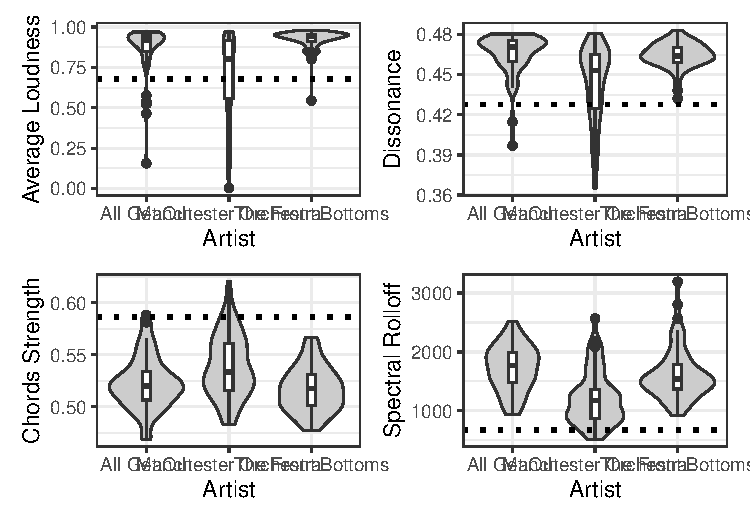
\includegraphics[width=\maxwidth]{figure/unnamed-chunk-3-1} 
\end{knitrout}
\caption{Sound Features}
\label{lyrical} 
\end{center}
\end{figure}
Figure 1 shows the four sound features with the black dotted line intersecting with the Manchester Orchestra in all four. This is replicated for the lyrical features in Figure 2 in the appendix. 

\columnbreak
\section{Discussion}
 This process is now automated and can be replicated with other files as well. This creates an efficient way to compare larger data sets of multiple artists or albums. The integrated, structured data frame allows for specific analysis to address research question in future work. 



%%%%%%%%%%%%%%%%%%%%%%%%%%%%%%%%%%%%%%%%%%%%%%%%%%%%%%%%%%%%%%%%%%%%%%%%%%%%%%%%
% Bibliography
%%%%%%%%%%%%%%%%%%%%%%%%%%%%%%%%%%%%%%%%%%%%%%%%%%%%%%%%%%%%%%%%%%%%%%%%%%%%%%%%
\vspace{2em}
\end{multicols} 
\begin{tiny}
\bibliography{bib.bib}
\end{tiny}

%%%%%%%%%%%%%%%%%%%%%%%%%%%%%%%%%%%%%%%%%%%%%%%%%%%%%%%%%%%%%%%%%%%%%%%%%%%%%%%%
% Appendix
%%%%%%%%%%%%%%%%%%%%%%%%%%%%%%%%%%%%%%%%%%%%%%%%%%%%%%%%%%%%%%%%%%%%%%%%%%%%%%%%
\pagebreak
\section{Appendix}

% latex table generated in R 4.4.2 by xtable 1.8-4 package
% Tue Feb 25 11:07:14 2025
\begin{table}[H]
\centering
\begingroup\small
\begin{tabular}{lll}
  \hline
artist & feature & description \\ 
  \hline
All Get Out & conj & Out of Range \\ 
  Manchester Orchestra & conj & Outlying \\ 
  The Front Bottoms & conj & Within Range \\ 
  All Get Out & Perception & Out of Range \\ 
  Manchester Orchestra & Perception & Within Range \\ 
  The Front Bottoms & Perception & Out of Range \\ 
  All Get Out & OtherP & Outlying \\ 
  Manchester Orchestra & OtherP & Outlying \\ 
  The Front Bottoms & OtherP & Within Range \\ 
  All Get Out & positivewords & Outlying \\ 
  Manchester Orchestra & positivewords & Outlying \\ 
  The Front Bottoms & positivewords & Within Range \\ 
   \hline
\end{tabular}
\endgroup
\caption{Lyrical Features} 
\end{table}




\begin{figure}[H]
\begin{center}
\begin{knitrout}
\definecolor{shadecolor}{rgb}{0.969, 0.969, 0.969}\color{fgcolor}
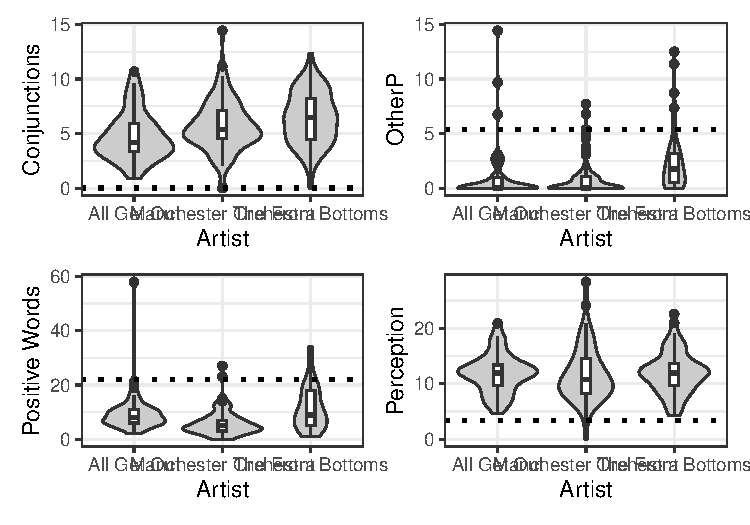
\includegraphics[width=\maxwidth]{figure/unnamed-chunk-5-1} 
\end{knitrout}
\caption{Lyrical Features}
\label{lyrical} 
\end{center}
\end{figure}

\begin{table}[ht]
\centering
\caption{Summary Table of 8 selected features}
\begin{tabular}{lrrrrll}
  \hline
artist & min & LF & UF & max & description & feature \\ 
  \hline
All Get Out & 935.91 & 701.91 & 2767.30 & 2520.04 & Out of Range & spectral\_rolloff \\ 
  Manchester Orchestra & 518.87 & 151.27 & 2083.17 & 2566.67 & Within Range & spectral\_rolloff \\ 
  The Front Bottoms & 927.04 & 740.58 & 2421.46 & 3190.29 & Out of Range & spectral\_rolloff \\ 
  All Get Out & 0.40 & 0.44 & 0.50 & 0.48 & Outlying & dissonance \\ 
  Manchester Orchestra & 0.37 & 0.36 & 0.53 & 0.48 & Within Range & dissonance \\ 
  The Front Bottoms & 0.43 & 0.44 & 0.49 & 0.48 & Out of Range & dissonance \\ 
  All Get Out & 0.16 & 0.70 & 1.10 & 0.97 & Outlying & average\_loudness \\ 
  Manchester Orchestra & 0.00 & 0.01 & 1.46 & 0.97 & Within Range & average\_loudness \\ 
  The Front Bottoms & 0.55 & 0.85 & 1.02 & 0.98 & Outlying & average\_loudness \\ 
  All Get Out & 0.47 & 0.47 & 0.58 & 0.59 & Outlying & chords\_strength \\ 
  Manchester Orchestra & 0.48 & 0.45 & 0.63 & 0.62 & Within Range & chords\_strength \\ 
  The Front Bottoms & 0.48 & 0.46 & 0.58 & 0.57 & Out of Range & chords\_strength \\ 
  All Get Out & 0.91 & -0.51 & 9.76 & 10.68 & Out of Range & conj \\ 
  Manchester Orchestra & 0.00 & 0.74 & 10.98 & 14.43 & Outlying & conj \\ 
  The Front Bottoms & 0.00 & -1.17 & 13.90 & 12.31 & Within Range & conj \\ 
  All Get Out & 4.67 & 4.14 & 18.91 & 20.89 & Out of Range & Perception \\ 
  Manchester Orchestra & 0.00 & -1.06 & 23.87 & 28.37 & Within Range & Perception \\ 
  The Front Bottoms & 4.27 & 3.74 & 19.66 & 22.56 & Out of Range & Perception \\ 
  All Get Out & 0.00 & -1.50 & 2.50 & 14.42 & Outlying & OtherP \\ 
  Manchester Orchestra & 0.00 & -1.64 & 2.73 & 7.69 & Outlying & OtherP \\ 
  The Front Bottoms & 0.00 & -3.48 & 7.20 & 12.50 & Within Range & OtherP \\ 
  All Get Out & 2.00 & -1.50 & 18.50 & 58.00 & Outlying & positivewords \\ 
  Manchester Orchestra & 0.00 & -3.00 & 13.00 & 27.00 & Outlying & positivewords \\ 
  The Front Bottoms & 1.00 & -14.50 & 37.50 & 34.00 & Within Range & positivewords \\ 
   \hline
\end{tabular}
\end{table}



\end{document}
